
\documentclass{article}
\usepackage{graphicx}
\usepackage{dot2texi}
\makeatletter
\@ifundefined{verbatim@out}{\newwrite\verbatim@out}{}
\makeatother
\usepackage{tikz}
\usetikzlibrary{shapes,arrows}
% \usepackage[pdf]{graphviz}
%\usepackage{feynmp}
\usepackage{subfigure}
\graphicspath{{figs/}}

\title{Deep Learning Notes}

\author{Peter Thompson}

\begin{document}

% TODO:
% add more on gradient saturation/relu/leaky relu
% Forward propagation
% BackPropagation
% Xavier Initialisation, He initialisation

\section{random notes}
Don't use sigmoid as an activation function. Tanh is generally superior, as it has a mean of zero (sigmoid has a mean of 0.5). Nonzero mean can make training more difficult in subsequent layers. Tanh has a mean of zero. May want a sigmoid as a final activation function (that is, in the output layer) when doing a binary classification problem.

relu is generally good.

\begin{figure}
% \begin{dot2tex}
% digraph G {
%     node [shape="circle"];
%     a_1 -> a_2 -> a_3 -> a_4 -> a_1;
%   }
% \end{dot2tex}
\begin{dot2tex}[mathmode]
digraph network1 {
rankdir=LR;
node [shape=circle];
subgraph inputlayer {
    node [shape=none];
    x_1 [label="x_1^2"];
    x_2 [label="x_2^2"];
    label="input layer";
    };
{x_1 x_2} -> {a_1 a_2 a_3 a_4} -> {o_1};
}
\end{dot2tex}
\caption{a network}
\end{figure}


% \begin{dot2tex}[mathmode]
% digraph network1 {
% rankdir=LR;
% subgraph inputlayer {
%     node [shape=none];
%     x1, x2 ;
%     label="input layer";
%     };
% {x1 x2} -> {a_1 a_2 a_3 a_4} -> {o_1};
% }
% \end{dot2tex}
% \caption{a network}
% \end{figure}

% subgraph inputlayer {
%     node [shape=none];
%     x1, x22 ;
%     label="input layer";
% };
% subgraph hiddenlayer{
%     node [shape=square];
%     a_1, a_2, a_3, a_4;
%     label="hidden layer";
% };
% subgraph outputlayer{
%     node [shape=circle];
%     o_1;
%     label="output layer";
% };
% {x_1 x_2} -> {a_1 a_2 a_3 a_4} -> {o_1};


\section{Notation}

\subsection{Matrix Dimensions/network layout/notation}
A network consists of $L$ layers. The $l$th layer contains $n_l$ neurons, or nodes. Each layer of the network consists of a number of neurons. Each layer of neurons applies an activation function to a vector of inputs $Z^l$ to produce a vector of outouts, or activations $A^l$, such that
\begin{eqnarray*}
A^l &=& f(Z^l) \\
& =& f(W^lA^{l-1} + b^l)
\end{eqnarray*}
Where $W^l$ is a matrix of weights for layer $l$ and $b^l$ is a vector of biases. The weight vector acts on the prior layer of activations, or the first layer acts on the raw inputs (the raw inputs,$X$, can be thought of as $A^{[0]}$. For $m$ training examples, $X$ has dimensions $(n_0,m)$, and each the weight matrix for each layer has dimension $(n^l,n^{l-1})$. 



Square brackets in the superscript denote the layer, for example, $A^{[l]}$ denotes the vector (or matrix) of activations (outputs) from the $l$th layer of the network. Round brackets in the superscript denote the training example (column for X,Y), such that $Z^{[l](i)}$ denotes the $ith$ column of the linearized inouts for the $l$th layer, squiggly brackets denote the mini batch number used in batched gradient descent, $A^{[l]\{k\}}$ are the activations for the $l$th layer in the $k$th mini batch.
Note that training epoch refers to the numer of traversals through the training dataset.




% A couple quick notes:
% \begin{itemize}
%     \item Each {\bf column} of the input, $X$, corresponds to an observation/example of the features. 
%     \item The weight matrix for layer $l$ should have dimensions $(n^l,n^{l-1})$, where $n^l$ is the number of nodes in layer $l$. The initial inputs, $X$, can be thought of as the activations of layer $l=0$. 
% \end{itemize}

\section{Loss and Cost functions}

Loss function is the loss/error associated with a single training example
Cost function is the loss computed over all examples

\subsection{logistic loss}

Think of $\hat{y}$ as the conditional probability $\hat{y}(x) = P(y=1|x)$. Based on our model, the probability $y=0$ is then $P(y=0|x) = 1 - \hat{y}$. For a single observation, these two outcomes can be summarised as
\begin{equation}
P(y|x) = \hat{y}^y(1-\hat{y})^{(1-y)}
\end{equation}
For a set of $(y_i,x_i)$ observations, $(Y,X)$, the likelihood of a given model is given by the product of the conditional probabilities
\begin{eqnarray*}
L(W|X) & = & P(Y|X) \\
& = & \prod_i P(y_i|x_i) \\
& = & \prod_i \hat{y}_i^{y_i}(1-\hat{y}_i)^{(1-y_i)}
\end{eqnarray*}
where $\hat{y}$ is described by our model, and is a function of $W$ and $x$.
% The above is for a single example. The likelihood (of parameters) for a given training set would be obtained from the product $\prod_i P(y_i|x_i)$, where $\hat(y)_i$ is a function of $x_i$.

The cost function from logistic loss can then be obtained from the negative log likelihood of $L(W|X)$ above
\begin{eqnarray*}
J(W,x) & = & - \log L(W|X) \\
 & = & \sum_i  (y_i-1) \log(1 - \hat{y}_i) - y_i \log(\hat{y}_i)
\end{eqnarray*}
The log of the product reduces to a sum over logs.

The cross entropy is a measure of dissimilarity between two different distributions, $p$ and $q$. 
\begin{equation}
H(p,q) = \sum_i p_i \log q_i
\end{equation}
The sum here runs over the values that $y$ can take (0 or 1), i.e. the dependant variable of the distributions $p$ and $q$. 

If we interpret $p$ as the distribution of $y$ and $q$ as the distribution of $\hat{y}$, then for our binary classification case we have $y \in \{0,1\}$, $p \in \{1-y,y\}$ and $q \in \{1-\hat{y},\hat{y}\}$.
The cross entropy for a single example is then
\begin{eqnarray*}
H(p,q) & = & - \sum_i p_i \log(q_i) \\
 & = & - \left( (1-y) \log (1-\hat{y}) + y \log \hat{y}\right)
\end{eqnarray*}
The cost function obtained by averaging $H(p,q)$ over all samples is then
\begin{eqnarray*}
J(W|X) & = & \frac{1}{N}\sum_n^N H(p_n,q_n) \\
 & = &  \frac{-1}{N} \left((1-y_n) \log (1-\hat{y}_n) + y \log \hat{y}_n\right)
\end{eqnarray*}
Which is equivalent (up to a constant factor) to the cost function obtained from logistic loss above. Minimising cross entropy in this case is equivalent to minimising the logistic loss, which results in the maximum likelihood estimate for the parameters $W$ of the model $\hat{y}$.


\section{activation functions and their derivatives}


\subsection{sigmoid}
Sigmoid used to be the default activation function, but in recent times ReLu has proven to be more popular/perform better. Sigmoid is still good for an output function (i.e. activation function in the output layer) in binary classification tasks.
The sigmoid function (or logit function) and its derivative are given by
\begin{eqnarray*}
\sigma(x) & = &\frac{1}{1 - e^{-x}} \\
\frac{d\sigma(x)}{dx} & = & \sigma(x)(1 - \sigma(x)) \\
\end{eqnarray*}

these are plotted below
\begin{figure}[tb]
\begin{centering}
\subfigure{
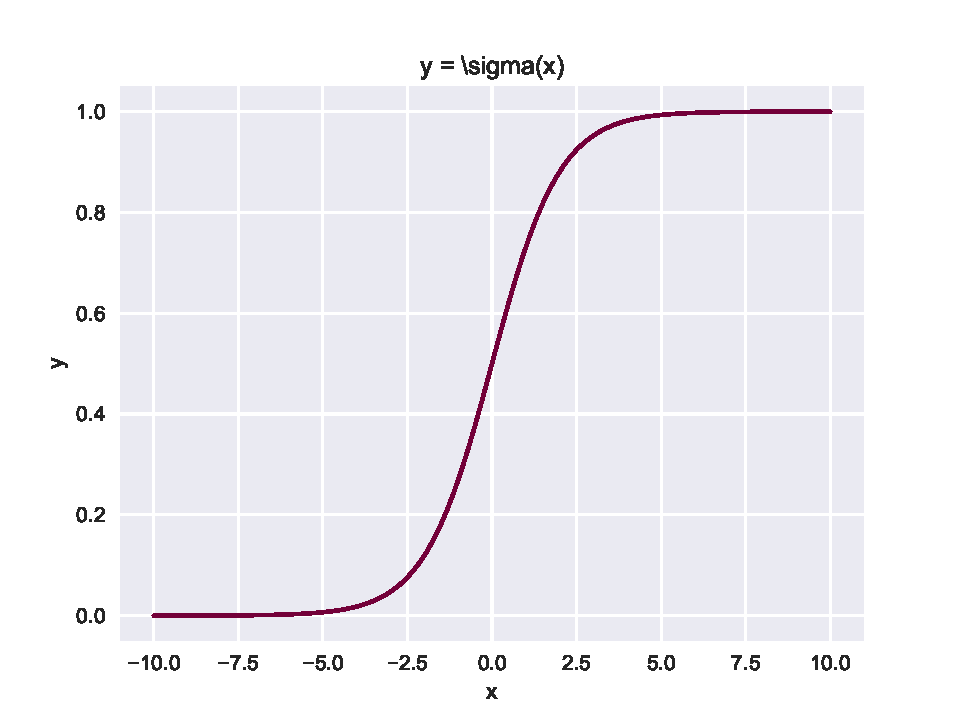
\includegraphics[width=0.45\linewidth,angle=0]{sigmoid.pdf}
% \caption{sigmoid activation function}
}
\subfigure{
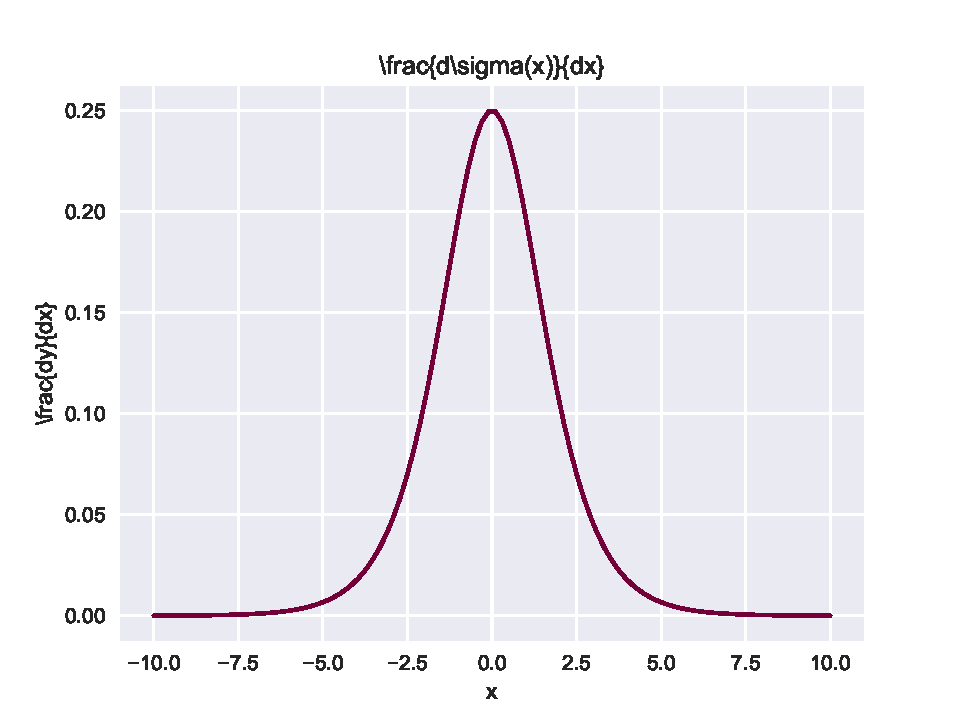
\includegraphics[width=0.45\linewidth,angle=0]{sigmoid_derivative.pdf}
% \caption{sigmoid derivative}
}
\end{centering}
\caption{sigmoid activation function and its derivative}

\end{figure}

\subsection{tanh}
Tanh is good. It's a nonlinear function, like sigmoid, but for zero input it returns zero output. The mean of this function (given uniform x) is zero, so it handles centred data very well ( zero input gives zero output).
The tanh function (sinh/cosh) and its derivative are given by
\begin{eqnarray*}
\mathrm{tanh}(x) & = &\frac{e^x\,-\, e^{-x}}{e^x\,+\, e^{-x}} \\
\frac{d\sigma(x)}{dx} & = & 1 - \mathrm{tanh}^2(x) 
\end{eqnarray*}

these are plotted below
\begin{figure}[tb]
\begin{centering}
\subfigure{
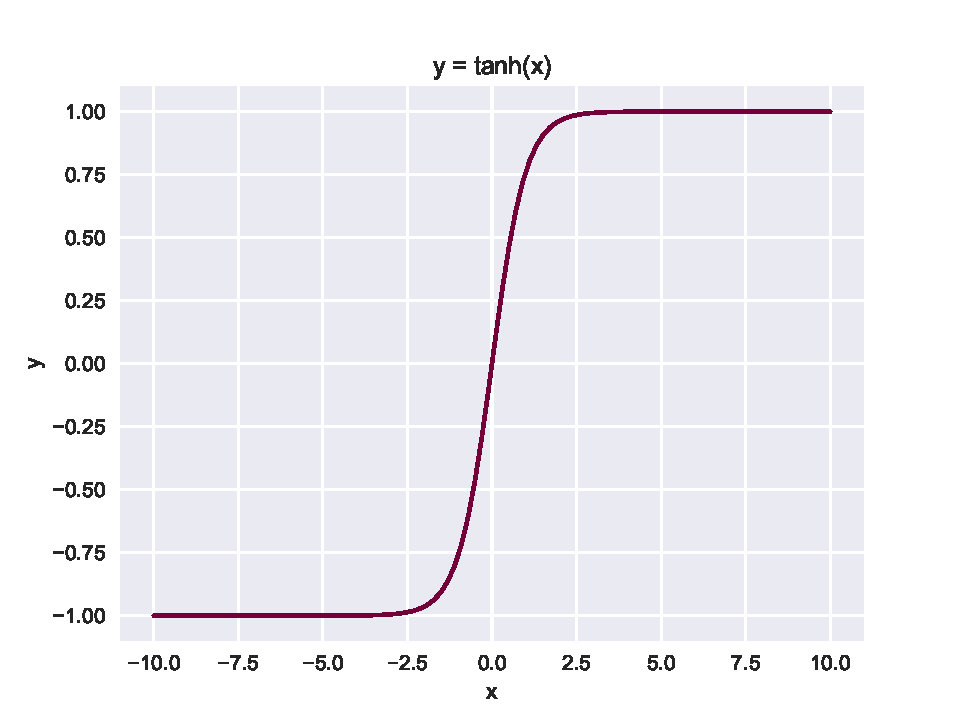
\includegraphics[width=0.45\linewidth,angle=0]{tanh.pdf}
}
\subfigure{
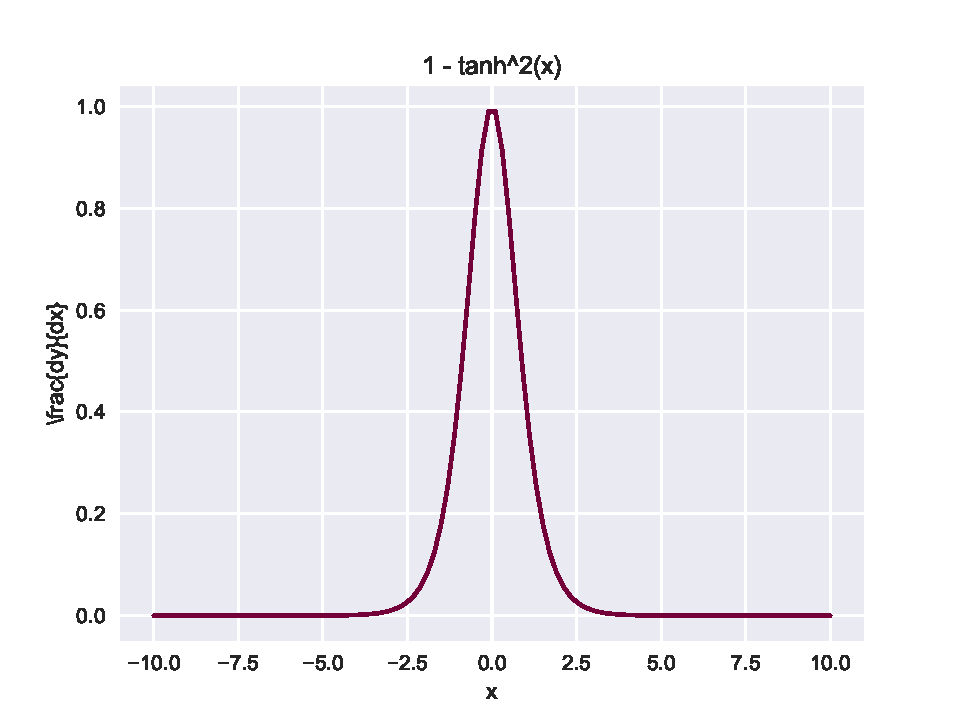
\includegraphics[width=0.45\linewidth,angle=0]{tanh_derivative.pdf}
% \caption{tanh derivative}
}
\end{centering}
\caption{tanh activation function and its derivative}
\end{figure}

\subsection{ReLu}
rectified linear unit. Max(0,x). This is a very popular activation, as it tends to give good results. Should in general be the first choice for an activation function (rather than sigmoid/tanh, though there may be cases where these perform better).
\begin{figure}[tb]
\begin{centering}
\subfigure{
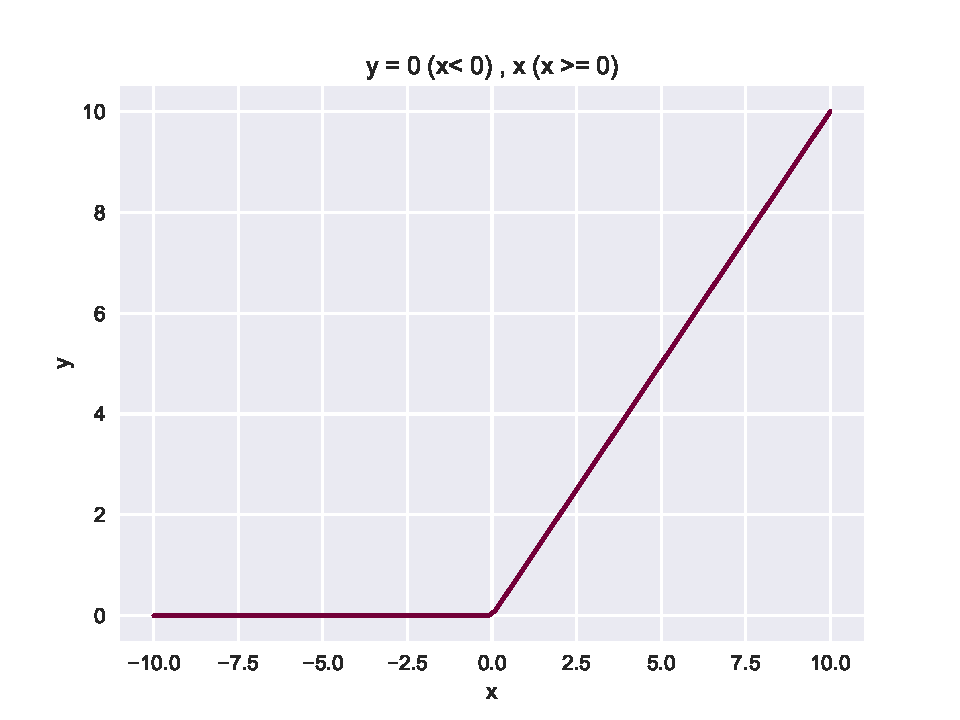
\includegraphics[width=0.45\linewidth,angle=0]{ReLu.pdf}
% \caption{tanh activation function}
}
\subfigure{
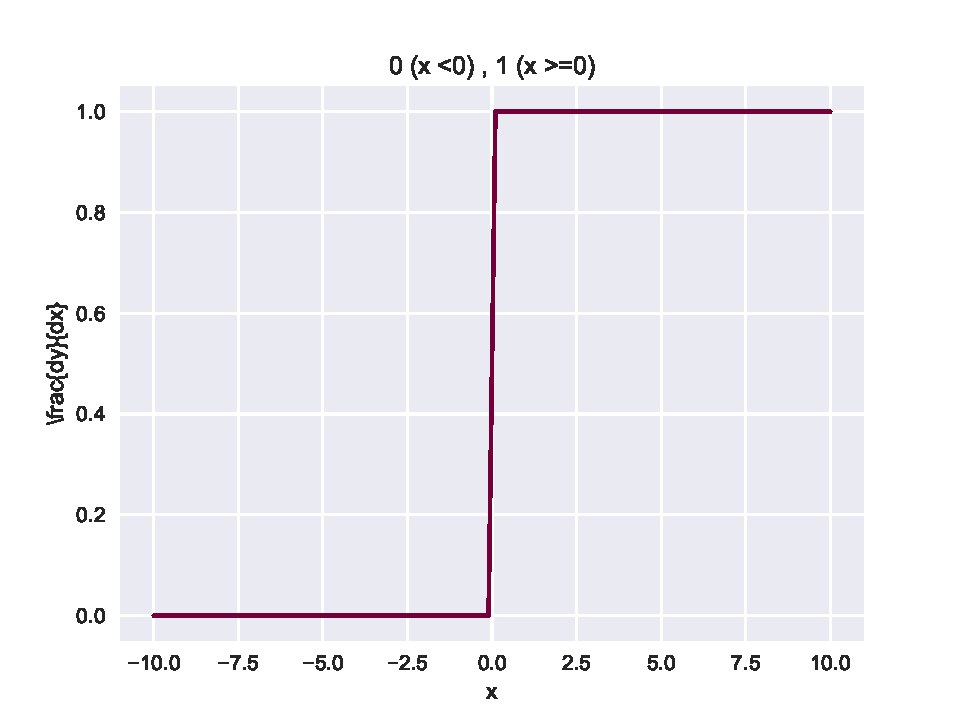
\includegraphics[width=0.45\linewidth,angle=0]{ReLu_derivative.pdf}
% \caption{tanh derivative}
}
\end{centering}
\caption{ReLu activation function and its derivative}
\end{figure}

\subsection{leaky ReLu}
Gradient saturation and such. If a Relu Network ever gets to a state where the inputs are large and negative, all the gradients will vanish, and the network will stop updating, it gets stuck. Leaky Relu has a very small (1\%) output for negative x, so the gradient never fully vanishes. It's a little more robust
\begin{figure}[tb]
\begin{centering}
\subfigure{
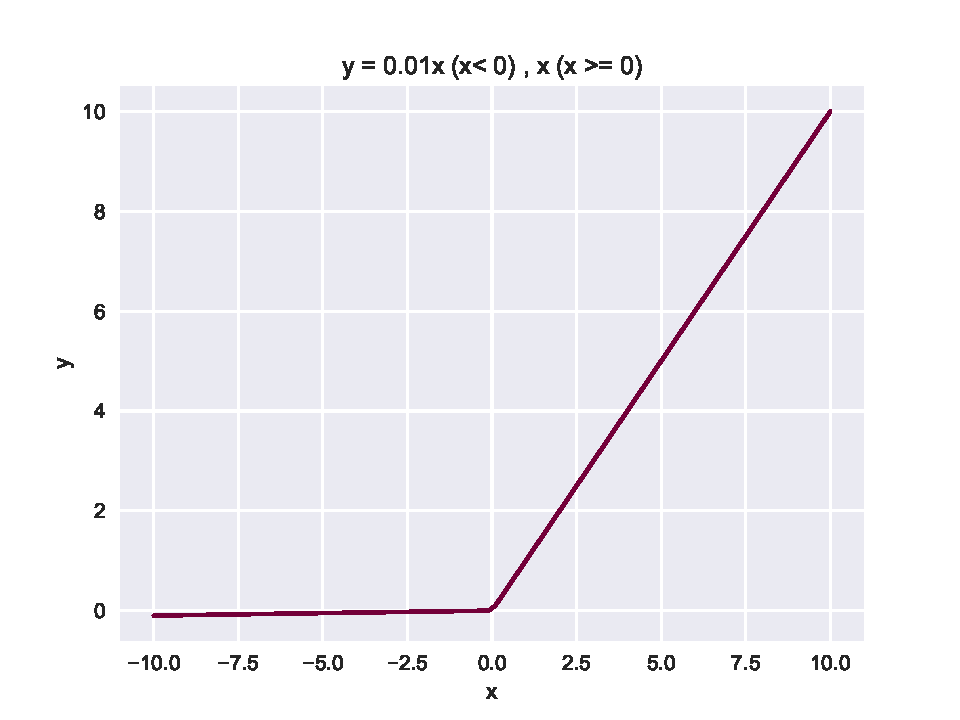
\includegraphics[width=0.45\linewidth,angle=0]{leaky_ReLu.pdf}
% \caption{tanh activation function}
}
\subfigure{
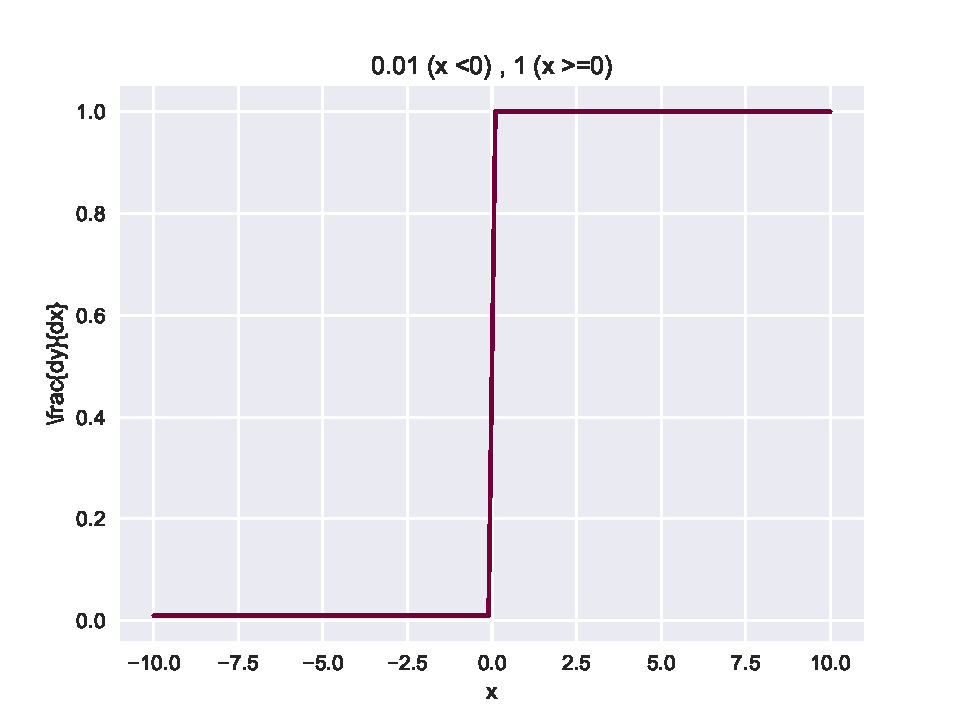
\includegraphics[width=0.45\linewidth,angle=0]{leaky_ReLu_derivative.pdf}
% \caption{tanh derivative}
} 
\end{centering}
\caption{Leaky Relu activation function and its derivative}

\end{figure}

\section{Initialisation}
Initialising weights to zero is a Bad Idea. 

\section{regularisation/tuning}
\subsection{dropout}
dropout is a form of regularisation where the outputs from certain nodes are randomly suppressed (set to zero). This can be thought of as an ensemble technique, instead of using a single network, an ensemble could be trained, each using different network configurations. Averaging over all members of the ensemble should reduce the variance of the model. Instead of actually training many different networks, the same structure is kept, but for each gradient descent iteration (forward prop and backward prop) the outputs of a set of randomly selected nodes are masked. 
 
In inverted dropout, each node is kept (not dropped) with probability $p$. In order to maintain the same expected value for activations, these are all scaled by the inverse of the keep probability, $1/p$, hence inverted dropout.
inverted dropout

\subsection{optimisation Methods}
\begin{itemize}
    \item {\bf Gradient Descent} - the usual. For each step, compute the activations for each training example. Compute the cost (over all training examples) and determine the gradients. Gradients are averaged over all training examples, and then a single step is taken. 
    \item {\bf Mini Batch Gradient descent} - Shuffle the training data, then divide into some number of batches. For each batch, compute the cost and average the gradients, then take a step. If there are $s$ batches, then $s$ iterations correspondf to one loop over the entire training set, or a single epoch.
    \item {\bf Stochastic Gradient descent} - Shuffle the training data, then randomly select a single example. compute the cost and gradient, then take a step. This is noisier, but the noise can improve performance in cases where the cost function (total) has a narrow valley like shape. Gradient descent would take many steps across the valley and back, and would take a long time to converge (if at all). The noise present in SGD means that the step is unlikely to be taken in the exactly optimal direction, so we move around the cost function more and don't get stuck going back and forth across the minimum. This also means that the steps can be computed quickly, we don't need to process a large number of examples to take a single step.
\end{itemize}
\subsection{ Momentum, RMSprop, Adam}
\subsubsection{exponentially weighted average}
\begin{equation}
v_t = \beta \theta_t + (1-\beta)v_{t-1}
\end{equation}
\subsubsection{momentum}
Instead of taking a minibatch gradient descent step using the gradients computed at iteration $t$, use a weighted average of the current gradient computation and the weighted gradient from the previous iteration
\subsubsection{RMSprop}

\subsubsection{Adam}

\section{Batch Normalisation}
In Logistic regression (for example), when feeding in features it can help to normalise things (centre and scale them). 
In neural networks, it would be good to normalise the inputs the inputs for each hidden layer, i.e. the activations $A^{[l-1]}$ of the preceding layer. This would make training the weights/biases of layer $l$ easier.

For batch normalisation, instead of normalising the activations, we normalise the linear input, $Z^{[l]}$
For the examples $i$ in a given batch, we compute
\begin{eqnarray}
\mu &=& \frac{1}{m} \sum_i Z^{(i)} \\
\sigma^2 &=& \frac{1}{m} \sum (Z^(i) - \mu)^2 \\
Z^{(i)}_\mathrm{norm} & = & \frac{Z^{(i)} - \mu}{\sqrt{\sigma^2 + \epsilon}}
\end{eqnarray}
Where $\epsilon$ is a small positive number. The normalised inputs $Z_\mathrm{norm}$ should thus have mean zero and unit variance. This seems good, but may not be ideal. We take a further step, and define
\begin{equation}
\tilde{Z}^{(i)} = \gamma Z^{(i)}_\mathrm{norm} + \beta
\end{equation}
where $\gamma$ and $\beta$ are tunable (hyper) parameters, that can be determined via backpropagation. This effectively tunes the mean and variance of the inputs $\tilde{Z}$ to the best value for the layer. This is done on a batch by batch basis.

For scoring, we might only be working with a single observation at a time. Also, tweaking network parameters based on test data is a Bad Idea. The batch normalisation parameters to be used when scoring should be computed while training. When computing the values for each batch, an exponentialy weighted averge of these parameters should be calculated. This average should be used when scoring.

\section{Structuring Machine Learning Projects}
\subsection{metrics}
There are satisficing and optimising metrics. For example, a system should run as fast as possible but use less thatn 10MB of memory. The memory requirement is a satisficing metric, either the solution satisfies the metric or it does not. The accuracy is an optimising metric, there is no hard limit on it, it should just be as high as possible.

Sometimes the evaluation metric can be tweaked depending on the situation. If there is a category of input that should not be miscategorised then these could receive a high weight in the evaluation metric. For example, consider an image classification task, for which we are interested in minimising the error. We really don't want to misclassify pornographic images as cats, so we assign a high weight to images that we know to be porn. An algorithm that performs well against this metric should be less likely to misclassify porn.

\subsection{Data distributions}

Generally, it is not ideal to train a model on a different distribution of data to what it will be exposed to when deployed. 
For a given project, there may be data available from a variety of sources. For example, consider image recognition in self driving cars. There may be many photos of the outdoors available from the internet, and maybe some more specific datasets consisting of car and road sign images, and maybe a small set of actual images taken by the camera of the car prototype. How to best make use of these depends on the size and relevance of these datasets.

The most relevant images are those taken by the car's camera during testing. We are most interested in how well our model performs on images like these. They should be included in the dev and test sets, and if there are enough of them then in training also. If the bulk of the training set comes from a different distribution (e.g. plentiful internet images), then it may not be beneficial to include all the car-camera images in there. 

If the car camera images are shared between test and dev sets, then this can introduce data-distribution errors. A difference between training and dev sets may generally be attributed to overfitting, but if training and dev are drawn from different distributions of data then this can be the source of the error. A training-dev set can be constructed by partitioning off a set of data from the same distribution as the training set. Comparing the training error rate with the training-dev error rate then gives some estimate of the model's variance. The difference between the training-dev and dev sets can then be attributed to data distribution differences, (assuming that the model is not overfitting to the dev set)

Bayes error rate - the lowest error rate acheivable
Human error rate - for tasks that humans are good at, generally considered a good approximation to Bayes rate
Training error rate > Human/Bayes rate - Model bias. Model should perform well on the training set. If not, use a more complex model.
Training-dev error rate > training error rate - Model is overfitting to the training set, get more data, use regularisation
Dev error rate > training-dev error rate - data distribution error. may need to augment training data, acquire more relevant training examples. Analyse dev set examples that are miscategorised, and try to figure out why the errors are occuring. Work on improving performance on the most significant sources of error.
Test error rate > dev error rate - overfit to dev set. Use regularisation, get more dev data.

dev set/test set, distributions

performing well on the training set by poorly on the dev set means we have overfit to our training data. We should increase regularisation, get more training data, 

\section{convolution layers}
\subsection{Convolutions}
In Image processing, convoloution takes a filters and moves it through (convolves it with) all possible positions in the input image. A filter of the form
\begin{equation}
f = \left[ \begin{array}{ccc}
1 & 0 & -1 \\
1 & 0 & -1 \\
1 & 0 & -1 
\end{array} \right]
\end{equation}
will identify ( give a strong output for) vertical edges. Cases where pixels in the rightmost column have a higher total value (are brighter) than pixels in the leftmost column will give a strong negative result, cases where the LHS are higher will give a positive result.

By setting the values of the filter elements, we can decide what sort of features (e.g. edges) we are looking for. An alternative is to leave all of the $f \times f$ elements as parameters, and have our deep learning model learn what sort of filters (or features) are appropriatte through backpropagation.


If the input image hasw dimension $n\times n$, and the filter has dimension $f \times f$, then the output of the convolution will be an array of dimension $n - f +1 \times n - f +1$. This is the number of ways that the filter can ``fit into'' the input image. This is called a ``valid'' convolution, it has two disadvantages in that it discards data around the edge of the input (or this data is not considered as often), and that the dimensions of the output are not equal to the input. An alternative is to pad the input image, i.e. add $p$ more pixels of synthetic data around the edges of the original image. With padding, the dimension of the output is given by $ n + 2p -f +1 \times n + 2p -f +1$, which is equal to $n$ if we choose $p = (f-1)/2$. 

Stride - sometimes we don't want (need) to apply an $f \times f$ filter to every unique $f \times f$ group of pixels in the input. A stride of $s$ means that we move the filter $s$ pixels over between each application of the filter. In this case, the output of the filter has dimension $(n + 2p - f)/s + 1 \times (n + 2p - f)/s + 1$  

\subsection{Convolutions over volume}

Images have generally 3 channels, rgb. We could have one filter for red edges, nother for green, and a third for blue. Instead, we could have a three dimensional filter ($f \times f \times n_c$) which acts on all colours and would produce a signal if it found vertical edges across any colours. We can also stack filters, so that we apply vertical and horizontal edge detection. In this case, our input image has size $n \times n \times n_c$, our filters have size $f\times f \times n_c$, and our output has size $ n-f+1 \times n-f+1 \times n_f$, where $n_f$ is the number of filters we have. The number of channels in the image and in the filter must match.

\subsection{Dimensions of a convolution layer}

As usual, square brackets in superscript refer to attributes of layer $l$:


\begin{tabular}{lr}
$f^{[l]}$ &  filter size \\ 
$p^{[l]}$ &  padding size (along each edge)\\ 
$s^{[l]}$ &  stride length\\ 
$n_c^{[l]}$ &  number of filters/channels\\ 
$a^{[l]}$ & activations\\
$n_w^{[l]}$ & number of pixels in each row\\
$n_h^{[l]}$ & number of pixels in each column\\
filter dimension &  $f^{[l]} \times f^{[l]} \times n_c^{[l-1]}$\\ 
input dimension & $n_h^{[l-1]} \times n_w^{[l-1]} \times n_c^{[l-1]}$  \\
output dimension &  $n_h^{[l]} \times n_w^{[l]} \times n_c^{[l]}$\\
$n_h^{[l]}$ & $\lfloor(n_h^{[l-1]} + 2 p^{[l]} - f^{[l]})/s^{[l]} + 1 \rfloor$ \\
$n_w^{[l]}$ & $\lfloor(n_w^{[l-1]} + 2 p^{[l]} - f^{[l]})/s^{[l]} + 1 \rfloor$ \\
\end{tabular}

Where $\lfloor x \rfloor$ denotes the floor of $x$ (round down to next integer value)
Note that the number of input image channels (colours) can be thought of as the number of filters in layer 0.

\subsection{Notable Networks}
\begin{itemize}
    \item AlexNet
    \item LeNet
    \item LMG16 (?)
\end{itemize}
\subsection{ResNets}

Residual networks - have an additional connection - there is an additional connection from one layer to a nodes in layers a few layers prior
For example, the activation at a given layer may have the form
\begin{eqnarray*}
a^{[l+2]} &= & g( z^{[l+2]} + a^{[l]} ) \\
& = & g( W^{[l+2]} a^{[l+1]} + b^{[l+2]} + a^{[l]} )
\end{eqnarray*}
There can be problems where the accuracy of a network degrades as the depth increases. The `shortcut' from the activation of layer $l$ to the input of layer $l+2$ means that the accuracy should not be worsened by the addition of the extra layer (if this were to happen, the coefficients $W^{[l+2]}$ should vanish) .

\subsection{object detection}
Train a net to classify objects. The output has 6 components: $[p_c, b_x, b_y, b_w, b_h, c]$. $p_c$ is the confidence, or score, for the detection, a high score indicates we are confident that we have detected an object. The quantities $b_x, b_y, b_w, b_w$ refer to the bounding box of the detected object, the coordinates of the centre of the box (x,y) and the width and height, respectively. $c$ is an encoding that represents the class of the object. This can be one-hot encoded, such that the output vector has dimension 5 + number of object classes.



\subsection{YOLO - you only look once}
\begin{itemize}
	\item bounding box - loss functions
	\item sliding window
	\item intersection over union
	\item anchor boxes/YOLO
\end{itemize}
{\bf go over this, add more detail}
Each grid has a number of anchor boxes associated with it. Each anchor box can identify an object. A give grid is responsible for identifying an object if that object's bounding box lies within the grid.
So Each grid looks for up to 5 objects. For each a bounding box is identified, as well as a class identifier and a confidence score. 

Once each grid has identified its objects, then the most relevant are kept. We don't want to identify the same image multiple times, so we take all objects of a given class and rank them by confidence. We only keep those for which the intersection over union is less than a given threshold, as this should ensure that identified objects are distinct.

\subsection{facial recognitino and one shot learning}


\subsection{neural style transfer}

\end{document}

